\appendix

%% ================================================================
%%  Appendix A: Model Construction
%% ================================================================
\section{Model Construction}
\label{app:model}

We formulate a one-dimensional Lagrangian model for the coupled thermo-chemo-poroelastic dynamics of a thermoresponsive gel slab undergoing an exothermic reaction. The conservative variables are the local swelling ratio $J(X,t)$, the reactant content per reference volume $Jc$, and the temperature $T(X,t)$; the solvent chemical potential is used as an algebraic mixed variable.

\subsection{Kinematics}

Consider a gel slab of reference (as-prepared) half-thickness $H_0$. We adopt a material (Lagrangian) coordinate $X\in[0,H_0]$, with $X=0$ denoting the symmetry plane and $X=H_0$ the free surface. The current position of a material point is $x(X,t)$, and the local volume ratio is
\begin{equation}
  J(X,t) = \frac{\partial x}{\partial X} > 0.
  \label{eq:J_def}
\end{equation}
In one dimension, $J$ is the local swelling ratio. The polymer volume fraction is a dependent variable determined by mass conservation of the network:
\begin{equation}
  \phi(X,t) = \frac{\pp}{J(X,t)},
  \label{eq:phi_J}
\end{equation}
where $\pp$ is the polymer volume fraction in the reference (as-prepared) state; $\pp=0.15$ corresponds to a gel that is $85\%$ solvent by volume at preparation. The current thickness of the slab is
\begin{equation}
  h(t) = x(H_0,t) = \int_0^{H_0} J(X,t)\,dX.
  \label{eq:thickness}
\end{equation}

\subsection{Governing equations}

\subsubsection{Swelling--permeation equation}

The evolution of $J$ is governed by solvent conservation:
\begin{equation}
  \frac{\partial J}{\partial t} = -\frac{\partial Q_s}{\partial X},
  \label{eq:J_evol}
\end{equation}
where $Q_s$ is the solvent flux relative to the polymer network, driven by chemical-potential gradients:
\begin{equation}
  Q_s = -M_s(J,T)\,\frac{\partial \mu_s}{\partial X}.
  \label{eq:Qs}
\end{equation}
Here $M_s(J,T)$ is the permeation mobility and $\mu_s$ is the solvent chemical potential.

\subsubsection{Reactant transport equation}

The reactant concentration $c(X,t)$ (moles per unit current total volume) evolves according to
\begin{equation}
  \frac{\partial (Jc)}{\partial t}
  + \frac{\partial N_c}{\partial X}
  = -J\,R(c,T,J),
  \label{eq:c_evol}
\end{equation}
with the total reactant flux
\begin{equation}
  N_c = c\,Q_s - D_c(J,T)\,\frac{\partial c}{\partial X}.
  \label{eq:Nc}
\end{equation}
The first term represents advective transport by the solvent flow, and the second term Fickian diffusion within the pore fluid. The effective diffusivity $D_c(J,T)$ depends on the local microstructure via $J$.

\subsubsection{Heat equation}

The temperature field satisfies
\begin{multline}
  C_\mathrm{eff}(J)\,\frac{\partial T}{\partial t}
  = \frac{\partial}{\partial X}\!\left(K_T(J)\,\frac{\partial T}{\partial X}\right)
  - \frac{\partial}{\partial X}\!\left(c_p^\ell\,T\,Q_s\right)
  \\
  + (-\Delta H_r)\,J\,R(c,T,J),
  \label{eq:T_evol}
\end{multline}
where $C_\mathrm{eff}(J)$ is the effective volumetric heat capacity,
$K_T(J)$ the effective thermal conductivity, $c_p^\ell$ the solvent
heat capacity per unit volume, and $-\Delta H_r > 0$ the exothermic
reaction enthalpy.  The three right-hand-side terms represent thermal
conduction, enthalpy advection by the solvent flow, and reaction heat
generation, respectively.

\subsection{Free energy and chemical potential}

The Helmholtz free-energy density per unit reference volume is written as
\begin{equation}
  \Psi(J,T) = \Psi_\mathrm{el}(J) + \Psi_\mathrm{mix}(\phi,T)
  + \frac{\kappa_J}{2}\left(\frac{\partial J}{\partial X}\right)^2,
  \label{eq:Psi}
\end{equation}
where $\phi = \pp/J$, and the three contributions are the elastic
energy of the network, the Flory--Huggins mixing energy, and a
gradient-energy regularization.

For the polymer network we adopt a neo-Hookean elastic energy
appropriate for uniaxial swelling in the slab geometry:
\begin{equation}
  \Psi_\mathrm{el}(J) = \frac{G}{2}
  \bigl(J^{2} - 1 - 2\ln J\bigr),
  \label{eq:Psi_el}
\end{equation}
where $G$ is the shear modulus of the reference-state network.

The mixing free-energy density takes the standard Flory--Huggins
form~\cite{Flory1953}:
\begin{equation}
  \Psi_\mathrm{mix}(\phi,T)
  = \frac{R_g T}{v_s}
  \Big[(1-\phi)\ln(1-\phi) + \chi(T,\phi)\,\phi(1-\phi)\Big],
  \label{eq:Psi_mix}
\end{equation}
with $R_g$ the gas constant, $v_s$ the solvent molar volume, and
the Flory--Huggins interaction parameter
\begin{equation}
  \chi(T,\phi) = \chi_0(T) + \chi_1\,\phi.
  \label{eq:chi}
\end{equation}
The temperature-dependent part $\chi_0(T)$ encodes the LCST
behavior of the gel; $\chi_1$ captures the leading
concentration dependence.

The solvent chemical potential is obtained as
$\mu_s = v_s\,\partial\Psi/\partial(1-\phi)\cdot
\partial(1-\phi)/\partial J$~\cite{Hong2008}.  Evaluating this
derivative yields the mixing contribution
\begin{equation}
  \frac{\mu_\mathrm{mix}}{R_g T/v_s}
  = \ln(1-\phi) + \phi + \chi(T,\phi)\,\phi^2
  - \phi^2(1-\phi)\,\frac{\partial\chi}{\partial\phi},
  \label{eq:mu_mix}
\end{equation}
so that the linear form~\eqref{eq:chi} gives
$\partial\chi/\partial\phi=\chi_1$.  The shorter expression without
this final term is retained only as an effective-osmotic comparison
closure, not as a strict free-energy derivative.
and the elastic contribution
\begin{equation}
  \frac{\mu_\mathrm{el}}{R_g T/v_s}
  = \frac{G\,v_s}{R_g T}
  \bigl(J - J^{-1}\bigr).
  \label{eq:mu_el}
\end{equation}
The full chemical potential, including the gradient-energy
regularization, is
\begin{equation}
  \mu_s = \mu_\mathrm{mix}(J,T) + \mu_\mathrm{el}(J)
  - \kappa_J\,\frac{\partial^2 J}{\partial X^2}.
  \label{eq:mu_s}
\end{equation}

\subsection{Reaction kinetics}

The volumetric reaction rate takes the Arrhenius form modulated by a collapse-dependent accessibility factor:
\begin{equation}
  R(c,T,J) = k_0\,c^n\,\exp\!\left(-\frac{E_a}{R_g T}\right) a(J),
  \label{eq:R}
\end{equation}
where $k_0$ is the pre-exponential factor, $n$ the reaction order, and $E_a$ the activation energy.

The activity factor $a(J)$ models the suppression of reaction due to reduced free solvent volume upon collapse:
\begin{equation}
  a(J) = A_\mathrm{min}+(1-A_\mathrm{min})\,
  \bar p^{\,m_\mathrm{act}}, \qquad
  \bar p=\mathrm{clip}\!\left[
    \frac{1-\phi}{1-\phi_\mathrm{ref}},0,1\right].
  \label{eq:aJ}
\end{equation}
When the gel collapses ($J\to\pp$, $\phi\to 1$), the activity approaches
the residual floor $A_\mathrm{min}$.  This is a phenomenological
porosity/accessibility closure rather than a microscopic derivation.

The effective transport coefficients similarly depend on the microstructure:
\begin{align}
  D_c(J) &= D_0\left[D_\mathrm{min}+(1-D_\mathrm{min})
  \bar p^{\,m_\mathrm{diff}}\right], \label{eq:Dc} \\
  M_s(J) &= M_0\,\bar p^{\,m_\mathrm{mob}}, \label{eq:Ms}
\end{align}
with optional Mackie--Meares and free-volume forms used only for
comparison.  Thus solute diffusion and solvent permeation are
suppressed but not forced to vanish in the collapsed state.

\subsection{Boundary conditions}

At the symmetry plane $X=0$:
\begin{equation}
  Q_s = 0, \qquad N_c = 0, \qquad \frac{\partial T}{\partial X} = 0.
  \label{eq:bc_sym}
\end{equation}

At the free surface $X=H_0$:

\paragraph{Solvent exchange.}
A Robin-type condition couples the surface chemical potential to the bath:
\begin{equation}
  Q_s = L_\mu\!\left(\mu_s - \mu_\mathrm{bath}\right),
  \label{eq:bc_mu}
\end{equation}
where $L_\mu$ is a surface transfer coefficient. In the limit of rapid equilibration, $\mu_s = \mu_\mathrm{bath}$.

\paragraph{Reactant supply.}
\begin{equation}
  N_c = k_c\,(c - c_b),
  \label{eq:bc_c}
\end{equation}
where $c_b$ is the constant bath concentration.

\paragraph{Heat exchange.}
\begin{equation}
  -K_T\,\frac{\partial T}{\partial X} = h_T\,(T - T_\infty),
  \label{eq:bc_T}
\end{equation}
where $h_T$ is the surface heat-transfer coefficient and $T_\infty$ the ambient temperature.

\paragraph{Mechanical boundary.}
The free surface is traction-free. In the $J$-formulation this is implicitly satisfied by the chemical-potential balance.

%% ================================================================
%%  Appendix B: Nondimensionalization
%% ================================================================
\section{Nondimensionalization}
\label{app:nondim}

\subsection{Scaling}

We introduce the following dimensionless variables. Length is scaled by the reference thickness:
\begin{equation}
  X = H_0\,\tilde{x}, \qquad \tilde{x}\in[0,1].
\end{equation}
The swelling ratio $J$ is already dimensionless. Reactant concentration is normalized by the bath value:
\begin{equation}
  c = c_b\,u.
\end{equation}
Temperature is measured relative to ambient, scaled by the adiabatic reaction temperature rise:
\begin{equation}
  T = T_\infty + \Delta T_*\,\theta,
  \qquad
  \Delta T_* = \frac{(-\Delta H_r)\,c_b}{C_*},
\end{equation}
where $C_*$ is a representative volumetric heat capacity.

The chemical potential is scaled by the thermal mixing energy:
\begin{equation}
  \mu_s = \mu_*\,m, \qquad \mu_* = \frac{R_g T_\infty}{v_s}.
\end{equation}

Time is scaled by the swelling/permeation time:
\begin{equation}
  \tau_s = \frac{H_0^2}{M_0\,\mu_*},
\end{equation}
where $M_0$ is a reference mobility. The solvent and reactant flux scales follow:
\begin{equation}
  Q_s = \frac{H_0}{\tau_s}\,q,
  \qquad
  N_c = \frac{c_b\,H_0}{\tau_s}\,n.
\end{equation}

Material functions are factored as reference value times dimensionless function:
\begin{align}
  M_s &= M_0\,\Ms(J,\theta), &
  D_c &= D_0\,\Ds_\mathrm{cur}(J,\theta), \\
  C_\mathrm{eff} &= C_*\,\Cs(J), &
  K_T &= K_*\,\Ks_\mathrm{cur}(J).
\end{align}
In the reference-coordinate equations below, the baseline closure
uses effective reference-coordinate coefficients
$\Ds_\mathrm{ref}$, $\Ks_\mathrm{ref}$, and $\Cs_\mathrm{ref}$.
When the tabulated coefficients are interpreted as current-space
material properties, the metric-corrected comparison uses
$\Ds_\mathrm{ref}=\Ds_\mathrm{cur}/J$,
$\Ks_\mathrm{ref}=\Ks_\mathrm{cur}/J$, and
$\Cs_\mathrm{ref}=J\Cs_\mathrm{cur}$.

\subsection{Dimensionless reaction rate}

Defining the reference reaction rate
\begin{equation}
  R_0 = k_0\,c_b^{\,n}\,\exp\!\left(-\frac{E_a}{R_g T_\infty}\right),
\end{equation}
we write $R = R_0\,\Rhat(u,\theta,J)$ with
\begin{equation}
  \Rhat(u,\theta,J)
  = u^n\,a(J)\,
  \exp\!\left[\frac{\Gamma_A\,\theta}{1+\varepsilon_T\,\theta}\right],
  \label{eq:Rhat}
\end{equation}
where
\begin{equation}
  \varepsilon_T = \frac{\Delta T_*}{T_\infty},
  \qquad
  \Gamma_A = \frac{E_a\,\Delta T_*}{R_g\,T_\infty^2}.
  \label{eq:epsT_GammaA}
\end{equation}
When $\varepsilon_T \ll 1$, this simplifies to $\Rhat \approx u^n\,a(J)\,e^{\Gamma_A\theta}$.

\subsection{Dimensionless chemical potential}

The dimensionless chemical potential is
\begin{equation}
  m = m_\mathrm{mix}(J,\theta) + m_\mathrm{el}(J) - \ell^2\,\frac{\partial^2 J}{\partial \tilde{x}^2},
  \label{eq:m_nondim}
\end{equation}
with the interface parameter
\begin{equation}
  \ell^2 = \frac{\kappa_J}{\mu_*\,H_0^2}.
\end{equation}

The mixing part retains the Flory--Huggins form (neglecting the
$T/T_\infty\approx 1+\varepsilon_T\theta\approx 1$ prefactor, valid
when $\varepsilon_T\ll 1$):
\begin{equation}
  m_\mathrm{mix} = \ln(1-\phi) + \phi + \chi(\theta,\phi)\,\phi^2
  -\phi^2(1-\phi)\,\frac{\partial\chi}{\partial\phi},
  \qquad \phi = \frac{\pp}{J},
  \label{eq:m_mix}
\end{equation}
with the dimensionless interaction parameter
\begin{equation}
  \chi(\theta,\phi) = \chi_\infty + S_\chi\,\theta + \chi_1\,\phi,
  \label{eq:chi_nondim}
\end{equation}
where $\chi_\infty = \chi_0(T_\infty)$ and the thermo-swelling sensitivity is
\begin{equation}
  S_\chi = \Delta T_*\left.\frac{d\chi_0}{dT}\right|_{T_\infty}.
  \label{eq:Schi}
\end{equation}
For the linear concentration dependence in Eq.~\eqref{eq:chi_nondim},
$\partial\chi/\partial\phi=\chi_1$.

The elastic contribution follows from Eq.~\eqref{eq:mu_el}:
\begin{equation}
  m_\mathrm{el} = \Omega_e\,(J - J^{-1}),
  \qquad
  \Omega_e = \frac{G\,v_s}{R_g\,T_\infty},
\end{equation}
measuring the network stiffness relative to the thermal mixing energy.

\subsection{Dimensionless governing equations}

Dropping tildes for clarity, the dimensionless system reads:

\paragraph{Swelling equation.}
\begin{equation}
  \frac{\partial J}{\partial t}
  = \frac{\partial}{\partial x}\!\left(\Ms(J,\theta)\,\frac{\partial m}{\partial x}\right),
  \label{eq:J_nondim}
\end{equation}

\paragraph{Chemical potential.}
\begin{equation}
  m = m_\mathrm{mix}(J,\theta) + m_\mathrm{el}(J) - \ell^2\,\frac{\partial^2 J}{\partial x^2},
  \label{eq:m_nondim_box}
\end{equation}

\paragraph{Reactant equation.}
\begin{equation}
  \frac{\partial(J u)}{\partial t}
  + \frac{\partial}{\partial x}\!\left(u\,q - \delta\,\Ds_\mathrm{ref}(J,\theta)\,\frac{\partial u}{\partial x}\right)
  = -\Da\,J\,\Rhat(u,\theta,J),
  \label{eq:u_nondim}
\end{equation}
where $q = -\Ms(J,\theta)\,\partial_x m$ and
\begin{equation}
  \delta = \frac{D_0}{M_0\,\mu_*}
\end{equation}
is the ratio of solute diffusion speed to solvent permeation speed.

The Damk\"ohler number, measuring reaction rate relative to swelling rate, is
\begin{equation}
  \Da = \tau_s\,k_0\,c_b^{\,n-1}\,\exp\!\left(-\frac{E_a}{R_g T_\infty}\right).
  \label{eq:Da}
\end{equation}

\paragraph{Heat equation.}
\begin{multline}
  \Cs_\mathrm{ref}(J)\,\frac{\partial\theta}{\partial t}
  = \alpha\,\frac{\partial}{\partial x}\!\left(\Ks_\mathrm{ref}(J)\,\frac{\partial\theta}{\partial x}\right)
  + \Da\,J\,\Rhat(u,\theta,J)
  \\
  - \alpha\,\Pe_T\,\frac{\partial}{\partial x}\!\left[(\Theta_\infty + \theta)\,q\right],
  \label{eq:theta_nondim}
\end{multline}
with
\begin{equation}
  \alpha = \frac{K_*\,\tau_s}{C_*\,H_0^2} = \frac{\tau_s}{\tau_T},
  \quad
  \Pe_T = \frac{c_p^\ell\,M_0\,\mu_*}{K_*},
  \quad
  \Theta_\infty = \frac{T_\infty}{\Delta T_*},
  \label{eq:thermal_params}
\end{equation}
where $\tau_T = C_*H_0^2/K_*$ is the thermal diffusion time.
When $\Pe_T \ll 1$, the convective term may be dropped.

\paragraph{Constraint.}
\begin{equation}
  \phi = \frac{\pp}{J}.
\end{equation}

\subsection{Dimensionless boundary conditions}

At $x=0$ (symmetry):
\begin{equation}
  q = 0, \qquad
  u\,q - \delta\,\Ds_\mathrm{ref}\,u_x = 0, \qquad
  \theta_x = 0.
  \label{eq:bc0_nondim}
\end{equation}

At $x=1$ (free surface):
\begin{align}
  q &= \Bi_\mu\,(m - m_b), \label{eq:bc1_mu} \\
  u\,q - \delta\,\Ds_\mathrm{ref}\,u_x &= \Bi_c\,(u - 1), \label{eq:bc1_c} \\
  -\alpha\,\Ks_\mathrm{ref}(J)\,\theta_x &= \Bi_T\,\theta, \label{eq:bc1_T}
\end{align}
where the surface Biot numbers for permeation and mass transfer are
\begin{equation}
  \Bi_\mu = \frac{L_\mu\,H_0}{M_0},
  \qquad
  \Bi_c = \frac{k_c\,H_0}{M_0\,\mu_*},
  \label{eq:Bi_mu_c}
\end{equation}
and the thermal exchange number is
\begin{equation}
  \Bi_T = \frac{h_T\,\tau_s}{C_*\,H_0}
  = \alpha\,\frac{h_T\,H_0}{K_*},
  \label{eq:Bi_T}
\end{equation}
which measures the surface heat loss rate directly on the swelling
timescale $\tau_s$.  The standard thermal Biot number
$h_T H_0/K_*=\Bi_T/\alpha$ is recovered by factoring out $\alpha$.

\subsection{Controlling parameter groups}

The oscillatory dynamics are governed by the following dimensionless groups:
\begin{itemize}
  \item $\Da$\,---\,Damk\"ohler number: strength of reaction heat source relative to swelling.
  \item $\alpha = \tau_s/\tau_T$\,---\,thermal diffusion relative to swelling.
  \item $S_\chi$\,---\,thermo-swelling sensitivity: how strongly temperature shifts the interaction parameter.
  \item $\Gamma_A$\,---\,Arrhenius feedback strength.
  \item $\delta$\,---\,solute diffusion to permeation ratio.
  \item $\ell$\,---\,interface regularization length.
  \item $\Bi_c$\,---\,surface reactant Biot number.
  \item $\Bi_T$\,---\,thermal exchange number (surface heat loss on the swelling timescale).
\end{itemize}
Together with the working-point parameters $\pp$ and $\chi_\infty$, these form the minimal set controlling the onset of self-oscillation. In physical terms, oscillation requires that the fast positive feedback (reaction $\to$ heating $\to$ collapse) and the slow negative feedback (collapse $\to$ transport suppression $\to$ cooling $\to$ re-swelling) operate on well-separated time scales.

%% ================================================================
%%  Appendix C: Dispersion Relation Derivation
%% ================================================================
\section{Homogeneous Diagnostic Derivation}
\label{app:lsa}

We derive the diagnostic matrix $\mathbf A(k)$ introduced in
Eq.~\eqref{eq:dispersion_matrix}.  The $k=0$ matrix $\mathbf A_0$
is obtained by volume-averaging the governing equations over the slab
domain and incorporating the Robin boundary fluxes as lumped
source/sink terms.  The $k^2$ and $k^4$ matrices $\mathbf D_2$ and
$\mathbf D_4$ collect local bulk-gradient corrections from a
point-wise normal-mode calculation.  This construction is not the
full finite-volume Jacobian eigenproblem with Robin boundary
conditions; it is a homogeneous stability diagnostic.

Starting from the mixed
formulation~\eqref{eq:mixed_J}--\eqref{eq:mixed_T}, the chemical
potential entering the swelling flux is
\begin{equation}
  m = f(J,\theta) - \ell^2 J_{\xi\xi},
\end{equation}
with $f(J,\theta)=m_\mathrm{mix}(J,\theta)+m_\mathrm{el}(J)$.
We perturb about the uniform base state with normal modes
$(\widehat J,\widehat u,\widehat\theta)^T e^{\sigma t+ik\xi}$
and define the partial derivatives
\begin{subequations}
\begin{align}
  f_J &= \left.\frac{\partial f}{\partial J}\right|_0, &
  f_\theta &= \left.\frac{\partial f}{\partial \theta}\right|_0,
  \\
  R_J &= \left.\frac{\partial \Rhat}{\partial J}\right|_0, &
  R_u &= \left.\frac{\partial \Rhat}{\partial u}\right|_0,
  \\
  R_\theta &= \left.\frac{\partial \Rhat}{\partial \theta}\right|_0,
\end{align}
\end{subequations}
and the base-state transport coefficients
\begin{subequations}
\begin{align}
  \Ms_0 &= \Ms(J_0,\theta_0), &
  \Ds_0 &= \delta\,\Ds_\mathrm{ref}(J_0,\theta_0),
  \\
  \Ks_0 &= \alpha\,\Ks_\mathrm{ref}(J_0), &
  \Cs_0 &= \Cs_\mathrm{ref}(J_0).
\end{align}
\end{subequations}

The $k=0$ matrix $\mathbf A_0$ contains the reaction and
boundary-exchange terms:
\begin{equation}
  \mathbf A_0 =
  \begin{bmatrix}
    a_{11} & 0 & a_{13} \\
    a_{21} & a_{22} & a_{23} \\
    a_{31} & a_{32} & a_{33}
  \end{bmatrix},
  \label{eq:A0}
\end{equation}
with entries
\begin{subequations}
\label{eq:A0_entries}
\begin{align}
  a_{11} &= -\Bi_\mu f_J, \qquad
  a_{13} = -\Bi_\mu f_\theta, \\
  a_{21} &= \frac{u_0\Bi_\mu f_J
             - \Da(\Rhat_0 + J_0R_J)}{J_0}, \\
  a_{22} &= \frac{-\Bi_c - \Da J_0 R_u}{J_0}, \\
  a_{23} &= \frac{u_0\Bi_\mu f_\theta
             - \Da J_0 R_\theta}{J_0}, \\
  a_{31} &= \frac{\Da(\Rhat_0 + J_0R_J)}{\Cs_0}, \quad
  a_{32} = \frac{\Da J_0 R_u}{\Cs_0}, \\
  a_{33} &= \frac{-\Bi_T + \Da J_0R_\theta}{\Cs_0}.
\end{align}
\end{subequations}
Note that $a_{12}=0$ because the swelling equation does not depend
directly on the reactant concentration.

The $k^2$ contribution collects diffusive transport:
\begin{equation}
  \mathbf D_2 =
  \begin{bmatrix}
    -\Ms_0 f_J & 0 & -\Ms_0 f_\theta \\
    0 & -\Ds_0/J_0 & 0 \\
    0 & 0 & -\Ks_0/\Cs_0
  \end{bmatrix}.
  \label{eq:D2}
\end{equation}
The $(1,1)$ entry $-\Ms_0 f_J$ changes sign when $f_J<0$ (spinodal
region), acting as a negative diffusivity for~$J$.

The only $k^4$ contribution arises from the Cahn--Hilliard
regularization:
\begin{equation}
  \mathbf D_4 =
  \begin{bmatrix}
    -\Ms_0\ell^2 & 0 & 0 \\
    0 & 0 & 0 \\
    0 & 0 & 0
  \end{bmatrix}.
  \label{eq:D4}
\end{equation}
Together, $\mathbf A(k) = \mathbf A_0 + k^2\mathbf D_2 +
k^4\mathbf D_4$ yields a $3\times 3$ eigenvalue problem for each
wavenumber~$k$.


%% ================================================================
%%  Appendix D: Numerical Method
%% ================================================================
\section{Numerical Method}
\label{app:numerics}

We describe a cell-centered finite-volume spatial discretization for the
dimensionless system derived in Appendix~\ref{app:nondim}.  Time
integration uses the implicit BDF method provided by
\textsc{scipy.integrate.solve\_ivp}: the spatial operators below
define the right-hand side of the resulting ODE system (method of
lines).  In the notation below, superscript~$n$ denotes the current
time level and~$n\!+\!1$ the new level; starred quantities
($\Ms_i^*$, $\theta_i^*$, $\Cs_i^*$) are evaluated at the most
recent available state, and $\sharp$-quantities ($J_i^\sharp$,
$u_i^\sharp$) at the values from the preceding fractional stage when
operator splitting is used.

\subsection{Mixed formulation}

To avoid discretizing fourth-order derivatives directly, we introduce the auxiliary variables $m$, $q$, $n$, and $h$ and write the system as
\begin{align}
  J_t + q_x &= 0, & q &= -\Ms_\mathrm{ref}(J,\theta)\,m_x, \label{eq:mixed_J} \\
  m &= f(J,\theta) - \ell^2\,J_{xx}, \label{eq:mixed_m} \\
  (Ju)_t + n_x &= -\Da\,J\,\Rhat, & n &= u\,q - \delta\,\Ds_\mathrm{ref}(J,\theta)\,u_x, \label{eq:mixed_u} \\
  \Cs_\mathrm{ref}(J)\,\theta_t + h_x &= \Da\,J\,\Rhat, & h &= -\alpha\,\Ks_\mathrm{ref}(J)\,\theta_x, \label{eq:mixed_T}
\end{align}
where $f(J,\theta) = m_\mathrm{mix}(J,\theta) + m_\mathrm{el}(J)$. This mixed form requires only $C^0$ regularity (no second-derivative continuity) and naturally accommodates Robin boundary conditions.

\subsection{Spatial discretization}

We use a uniform mesh of $N$ cells:
\begin{equation}
  \Delta x = \frac{1}{N},
  \qquad
  x_i = \left(i - \tfrac{1}{2}\right)\Delta x,
  \quad i = 1,\dots,N.
  \label{eq:mesh}
\end{equation}
Face positions are $x_{i+1/2} = i\,\Delta x$ for $i=0,\dots,N$. Cell-centered unknowns are $J_i,\,m_i,\,u_i,\,\theta_i$; face fluxes are $q_{i+1/2},\,n_{i+1/2},\,h_{i+1/2}$.

\subsubsection{Swelling equation}

The conservative update reads
\begin{equation}
  \frac{J_i^{n+1} - J_i^{n}}{\Delta t}
  + \frac{q_{i+1/2}^{n+1} - q_{i-1/2}^{n+1}}{\Delta x} = 0,
  \label{eq:disc_J}
\end{equation}
with the face flux
\begin{equation}
  q_{i+1/2}^{n+1}
  = -\Ms_{i+1/2}^{*}\,
  \frac{m_{i+1}^{n+1} - m_i^{n+1}}{\Delta x}.
  \label{eq:disc_q}
\end{equation}
The face mobility $\Ms_{i+1/2}^{*}$ is evaluated using the harmonic mean
\begin{equation}
  \Ms_{i+1/2}^{*}
  = \frac{2\,\Ms_i^{*}\,\Ms_{i+1}^{*}}{\Ms_i^{*} + \Ms_{i+1}^{*}},
  \label{eq:harm_mean}
\end{equation}
which is more robust than arithmetic averaging for degenerate mobilities.

\subsubsection{Chemical potential}

The discrete chemical potential is
\begin{equation}
  m_i^{n+1}
  = f(J_i^{n+1},\theta_i^{*})
  - \ell^2\,\frac{J_{i+1}^{n+1} - 2J_i^{n+1} + J_{i-1}^{n+1}}{\Delta x^2},
  \label{eq:disc_m}
\end{equation}
where the natural boundary condition $\partial_x J = 0$ is imposed via ghost cells:
\begin{equation}
  J_0^{n+1} = J_1^{n+1}, \qquad J_{N+1}^{n+1} = J_N^{n+1}.
  \label{eq:ghost_J}
\end{equation}

\subsubsection{Reactant equation}

To preserve conservation, we update the product $W_i = J_i\,u_i$:
\begin{equation}
  \frac{W_i^{n+1} - W_i^{n}}{\Delta t}
  + \frac{n_{i+1/2}^{n+1} - n_{i-1/2}^{n+1}}{\Delta x}
  = -\Da\,J_i^{\sharp}\,\Rhat(u_i^{\sharp},\theta_i^{\sharp},J_i^{\sharp}),
  \label{eq:disc_W}
\end{equation}
followed by reconstruction $u_i^{n+1} = W_i^{n+1}/J_i^{n+1}$.

The reactant face flux combines upwind advection and central diffusion:
\begin{equation}
  n_{i+1/2}^{n+1}
  = q_{i+1/2}^{n+1}\,u_{i+1/2}^\mathrm{up}
  - \delta\,\Ds_{\mathrm{ref},i+1/2}^{*}\,
  \frac{u_{i+1}^{n+1} - u_i^{n+1}}{\Delta x},
  \label{eq:disc_n}
\end{equation}
where the upwind value is
\begin{equation}
  u_{i+1/2}^\mathrm{up}
  = \begin{cases}
    u_i^{n+1}, & q_{i+1/2}^{n+1} \ge 0, \\[4pt]
    u_{i+1}^{n+1}, & q_{i+1/2}^{n+1} < 0.
  \end{cases}
  \label{eq:upwind}
\end{equation}
Upwinding is essential to suppress spurious oscillations when advection dominates over diffusion.

\subsubsection{Heat equation}

The thermal update is
\begin{equation}
  \Cs_i^{*}\,\frac{\theta_i^{n+1} - \theta_i^{n}}{\Delta t}
  + \frac{h_{i+1/2}^{n+1} - h_{i-1/2}^{n+1}}{\Delta x}
  = \Da\,J_i^{\sharp}\,\Rhat(u_i^{\sharp},\theta_i^{\sharp},J_i^{\sharp}),
  \label{eq:disc_theta}
\end{equation}
with the heat flux (neglecting enthalpy advection)
\begin{equation}
  h_{i+1/2}^{n+1}
  = -\alpha\,\Ks_{\mathrm{ref},i+1/2}^{*}\,
  \frac{\theta_{i+1}^{n+1} - \theta_i^{n+1}}{\Delta x}.
  \label{eq:disc_h}
\end{equation}

\subsection{Boundary conditions}

At the left boundary ($x=0$):
\begin{equation}
  q_{1/2}^{n+1} = 0,
  \qquad
  n_{1/2}^{n+1} = 0,
  \qquad
  h_{1/2}^{n+1} = 0.
  \label{eq:disc_bc0}
\end{equation}

At the right boundary ($x=1$), the Robin conditions become face fluxes:
\begin{align}
  q_{N+1/2}^{n+1} &= \Bi_\mu\,(m_N^{n+1} - m_b), \label{eq:disc_bc1_q} \\
  n_{N+1/2}^{n+1} &= \Bi_c\,(u_N^{n+1} - 1), \label{eq:disc_bc1_n} \\
  h_{N+1/2}^{n+1} &= \Bi_T\,\theta_N^{n+1}. \label{eq:disc_bc1_h}
\end{align}

\subsection{Time integration}

The primary integration strategy is the method of lines (MOL): the
spatial discretization above defines a system of $4N$ coupled ODEs
that is advanced in time by the variable-order implicit BDF solver
(\textsc{scipy.integrate.solve\_ivp} with \texttt{method='BDF'} and
a precomputed Jacobian sparsity pattern).  Adaptive time stepping
and error control are handled by the library.

For parameter regimes where the BDF solver encounters difficulties,
an alternative IMEX operator-splitting strategy is available, in
which each time step proceeds sequentially:

\paragraph{Stage 1: Swelling $(J,m,q)$.}
Given $(J^n, u^n, \theta^n)$, solve the coupled nonlinear system~\eqref{eq:disc_J}--\eqref{eq:disc_m} for $(J^{n+1}, m^{n+1}, q^{n+1})$ using Newton iteration. The mobility and thermodynamic function $f$ are evaluated at the current iterate $(J^{(k)},\theta^{(k)})$.

\paragraph{Stage 2: Reactant $(W,u)$.}
With $J^{n+1}$ and $q^{n+1}$ known, solve the linear (or mildly nonlinear) system~\eqref{eq:disc_W}--\eqref{eq:disc_n} for $W^{n+1}$, then recover $u^{n+1} = W^{n+1}/J^{n+1}$. Diffusion is treated implicitly; the reaction source may be linearized about the current temperature.

\paragraph{Stage 3: Temperature $(\theta)$.}
With $J^{n+1}$ and $u^{n+1}$ known, solve the implicit heat equation~\eqref{eq:disc_theta}--\eqref{eq:disc_h} for $\theta^{n+1}$. If the Arrhenius source term is stiff, a Newton linearization of the source with respect to $\theta$ is applied.

\subsection{Fully coupled Newton formulation}

For problems requiring tight coupling, the unknowns are assembled
into a single vector
\begin{multline}
  \bm{Y} = (J_1,\dots,J_N,\;m_1,\dots,m_N,\\
  W_1,\dots,W_N,\;\theta_1,\dots,\theta_N)^T
\end{multline}
and the residual vector $\bm{R}(\bm{Y})$ collects all discrete equations~\eqref{eq:disc_J}--\eqref{eq:disc_h} with boundary conditions~\eqref{eq:disc_bc0}--\eqref{eq:disc_bc1_h}. The system is solved by Newton's method:
\begin{equation}
  \bm{J}_\mathrm{ac}\,\delta\bm{Y} = -\bm{R}(\bm{Y}^{(k)}),
  \qquad
  \bm{Y}^{(k+1)} = \bm{Y}^{(k)} + \delta\bm{Y},
\end{equation}
where $\bm{J}_\mathrm{ac}$ is the Jacobian matrix. Because all couplings are local in one dimension, the Jacobian is sparse and banded; its sparsity pattern is precomputed and supplied to the BDF integrator for efficient graph-coloring-based finite-difference Jacobian evaluation.

\subsection{Implementation notes}

\begin{enumerate}
  \item The conserved variable $W = Ju$ must be used for the reactant update, not a non-conservative discretization of $u$ alone. This ensures that boundary supply and internal reaction remain in balance even during rapid swelling or collapse.
  \item Upwind discretization of the advective flux $u\,q$ is mandatory, not optional. Central differencing produces non-physical oscillations whenever $|q|\,\Delta x / (\delta\,\Ds_\mathrm{ref}) \gg 1$.
  \item The fourth-order swelling--chemical-potential system must be split into two second-order equations (mixed form). Direct discretization of $J_{xxxx}$ leads to wider stencils and difficulties with natural boundary conditions.
\end{enumerate}


\section{Spinodal Decomposition Verification}
\label{app:spinodal}

The finite-wavenumber instability identified in
Sec.~\ref{sec:lsa} corresponds to spinodal decomposition of the gel
within the Flory--Huggins two-phase region.  To verify that this mode
is a genuine feature of the model---not merely an artifact of the
linearization---we perform a direct numerical simulation of the
pure Cahn--Hilliard dynamics: the reaction is switched off ($\Da=0$),
the temperature is held fixed at $\theta=1.5$ (above the LCST), and
no-flux boundary conditions are imposed at both ends.

The simulation starts from a spatially uniform collapsed state
$J_0=0.30$ ($\phi=0.50$) with small random perturbations
($\delta J/J_0\sim 0.1\%$), using $N=301$ grid points and
$\ell=0.01$.  At this state, $f_J=-1.76<0$, confirming that the
uniform state is inside the spinodal.  The predicted
fastest-growing wavenumber is
$k^\ast=\sqrt{-f_J/(2\ell^2)}\approx 94$, corresponding to a
domain spacing $\lambda^\ast\approx 0.067\,H_0$.  The maximum
growth rate is $\sigma^\ast=\Ms_0 f_J^2/(4\ell^2)\approx 3850$,
where $\Ms_0=(1-\phi)^{m_\mathrm{mob}}=0.50$ is the base-state
mobility.

Figure~\ref{fig:spinodal} shows the result.  The initially uniform
state spontaneously separates into alternating swollen
($J\approx 0.7$) and collapsed ($J\approx 0.2$) domains within
$\tau\lesssim 0.1$ [Fig.~\ref{fig:spinodal}(a,b)].  The Fourier
amplitude at $k\approx k^\ast$ [Fig.~\ref{fig:spinodal}(c)] grows
exponentially at the predicted rate $2\sigma^\ast$ over five orders
of magnitude before saturating as the system enters the nonlinear
regime.  The full Fourier spectrum
[Fig.~\ref{fig:spinodal}(d)] confirms that the dominant
wavenumber during the linear growth phase ($\tau\lesssim 0.003$)
peaks near the predicted $k^\ast$; at later times, the spectrum
shifts to lower $k$ as domains coarsen through coalescence.

This verification establishes two points: (i)~the model
faithfully captures Cahn--Hilliard spinodal physics with
quantitative agreement between the linear prediction and the
nonlinear simulation; (ii)~the spinodal mode operates on a
timescale ($\sigma^{\ast\,-1}\sim 3\times 10^{-4}\,\tau$) that
is three orders of magnitude faster than the Hopf oscillation
period ($T\sim 20\,\tau$), explaining why it does not interfere
with the self-sustained oscillation dynamics when the reaction is
active.

\begin{figure}[tbp]
  \centering
  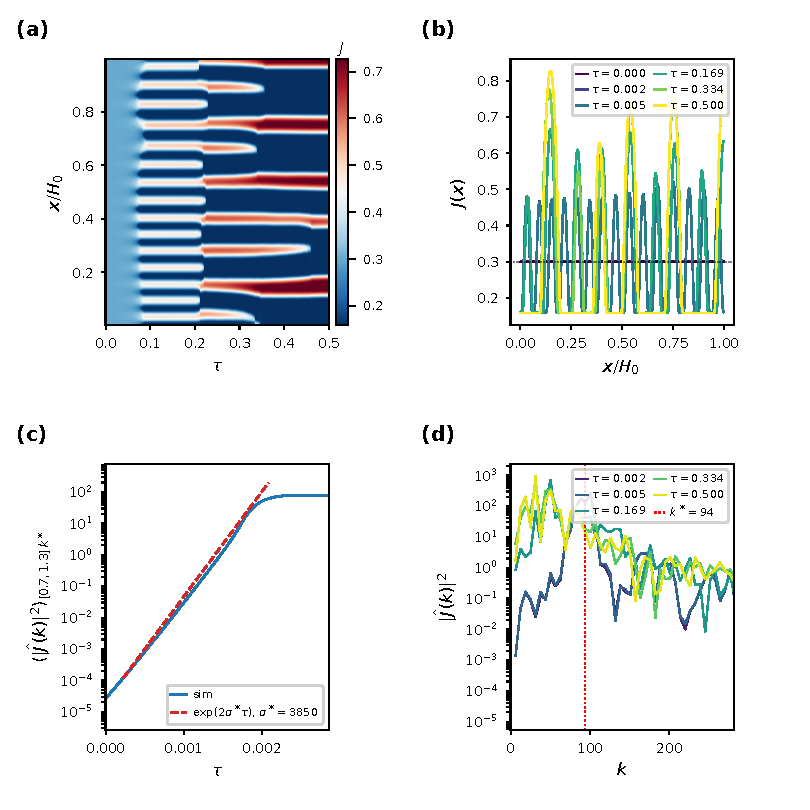
\includegraphics[width=\columnwidth]{figures/fig09/Figure/fig7/fig7.pdf}
  \caption{Spinodal decomposition in the gel model with $\Da=0$
    (no reaction), $\theta=1.5$ (fixed), $J_0=0.30$,
    $\ell=0.01$, $N=301$, no-flux boundaries.
    \textbf{(a)}~Kymograph of $J(x,\tau)$ showing spontaneous
    domain formation and subsequent coarsening.
    \textbf{(b)}~Spatial profiles at selected times.
    \textbf{(c)}~Fourier amplitude $|\hat J(k^*)|^2$ averaged
    over $k\in[0.7k^*,1.3k^*]$; the predicted exponential growth
    at rate $2\sigma^*$ (red dashed) matches the simulation over
    five decades before nonlinear saturation.
    \textbf{(d)}~Fourier power spectrum $|\hat J(k)|^2$; the
    earliest curves peak near $k^*\!\approx 94$ (red dotted),
    shifting to lower $k$ during coarsening.}
  \label{fig:spinodal}
\end{figure}

